% Short ORIGINAL RESEARCH article track, adapted for SN Computer Science.
% This file does NOT replace the archival full paper in main.tex.
% Rebuild the figures from cached CSV/JSON; no benchmarks are rerun.
\documentclass[pdflatex,sn-mathphys-ay]{sn-jnl}
\usepackage{graphicx}
\usepackage{amsmath,amssymb,amsfonts}
\usepackage{booktabs}
\usepackage{url}
\newcommand{\R}{\mathbb R}
\newcommand{\tr}{\operatorname{tr}}
\begin{document}
\title[Smoothness-first computational trend estimation]{Smoothness-indexed penalized trend estimation in Python: parameter-search coordinates, numerical backends, and reproducible comparisons}
\author*[1]{\fnm{Heriberto} \sur{Espino-Montelongo}}
\author[1]{\fnm{Daniela} \sur{Cort\'es-Toto}}
\affil*[1]{\orgname{Universidad de las Am\'ericas Puebla},
 \orgaddress{\city{San Andr\'es Cholula},\state{Puebla},\country{Mexico}}}

\abstract{Penalized least-squares (PLS) smoothing is established, but its practical computational behavior depends on the difference order, reference-difference mean, numerical solver, optimization coordinate and reuse of intermediate computations. We describe an open-source Python implementation that offers Guerrero's trace-based smoothness through a normalized, order-comparable coordinate $S$ while preserving familiar penalty-based selectors. The article derives the relationship between $S$ and $\lambda$, distinguishes matched-grid search from changes in candidate sets, and evaluates seven numerical backends under an archived 80,640-record Windows factorial design spanning five criteria and two reference means. An independent seed-paired study quantifies full-trend solver speed with bootstrap confidence intervals and Holm-adjusted comparisons; a separate float64 study evaluates four safeguarded inversion algorithms. Archived CO$_2$ and federal funds series illustrate selected smoothness, fitted trends at four difference orders, and historical extrapolation behavior. Results show that both numerical validity and the cost of reusing factorizations and mapped grids matter; no backend is universally fastest, and changing search coordinates does not change the underlying statistical criterion. A reproducible Python API, saved numerical evidence, and render-only graphics complete the implementation contribution.}
\keywords{penalized least squares, Whittaker--Henderson smoother, numerical algorithms, smoothness inversion, reproducible benchmarking, time series}
\maketitle

\section{Introduction}\label{sec:sncs-intro}
Finite-difference penalized least squares (PLS) provides a flexible way
to separate persistent variation from noise. The underlying estimator
and its history are well established in the work of Whittaker and
Guerrero \cite{whittaker1923graduation,guerrero2007penalized}.
Cort\'es-Toto et al.\ \cite{cortes2017smoothness} studied attained
trend smoothness when traditional CV, GCV, AICc and BIC select the
penalty. Efficient structured Whittaker--Henderson computation
has an extensive earlier literature \cite{weinert2007wh},
so neither diagonalization nor smoothness-controlled fitting
is presented here as a newly discovered mathematical method.

A modern Python user nevertheless confronts three distinct choices.
First, the difference order $d$ and reference difference mean
$\mu$ determine the geometry of the fitted trend. Second,
a statistical selector or a user-specified smoothness target
determines the amount of smoothing. Third, the numerical
backends and search coordinates determine the computational
cost of reaching that same fit. These three issues are
often conflated. Our software aims to make them explicit
and reproducible.

In particular, a raw penalty $\lambda$ cannot be compared across
difference orders as a universal smoothness scale. We expose
a version of Guerrero's trace-based smoothness index normalized
by the number of \emph{penalizable} coordinates, so that
$S\in[0,1]$ for all $1\le d<n$. This is a monotone rescaling
of an established quantity, not a new optimality score.
It is, however, a practical interface: a fixed target
$S$ can be requested directly, and existing CV/GCV/AICc/BIC
or conditional MLE searches can be expressed either in
$\lambda$ or in $S$. The choice matters for candidate
grids, scalar inverse costs, and factorization reuse.

The present contribution is therefore computational and
software-centered: (1) an auditable, reusable Python interface
that permits controlled smoothness as well as classical
criteria; (2) an exact distinction between matched and
unmatched parameter grids and their preparation costs;
(3) measured end-to-end comparisons over difference
orders, fixed means and selection criteria with
numerical-validity checks; (4) separate paired uncertainty
analysis and numerical-inversion accuracy measurements; and
(5) real-data fitted trends and reproducible figures
generated from immutable archived results.

For journal-level experimental organization, we draw on
the separation between time and quality in Berns et al.\
\cite{berns2022automated}, the interpretation of smoothing
trade-offs in Gauss et al.\ \cite{gauss2021skeleton}, and
explicit algorithmic comparisons in Cardoso et al.\
\cite{cardoso2025novelty}. These articles concern
different algorithms and are presentation comparators,
not claims about performance of our PLS software.

\section{From penalized least squares to a smoothness coordinate}
\label{sec:expanded-theory}
Let $y=(y_1,\dots,y_n)^\top$ denote equally spaced observations.
For $1\leq d<n$, define the $d$th forward-difference operator
$D_d\in\mathbb R^{(n-d)\times n}$, so $D_1\tau$ contains consecutive
increments and $D_2\tau$ contains consecutive differences of increments.
The order is not itself a smoothness magnitude: it defines which
local changes are penalized. With a reference difference mean
$\mu$, our fitted trend is
\begin{equation}
\widehat{\tau}_{\lambda,\mu}
=\arg\min_\tau\bigl\{\|y-\tau\|_2^2+
  \lambda\|D_d\tau-\mu\mathbf1\|_2^2\bigr\},\quad
  \lambda\ge0 .
\label{eq:expanded-pls}
\end{equation}
The normal equations give
\begin{equation}
(I+\lambda Q_d)\widehat\tau_{\lambda,\mu}
=y+\lambda\mu D_d^\top\mathbf1,\qquad Q_d=D_d^\top D_d.
\label{eq:expanded-normal}
\end{equation}
Since the objective is strictly convex for every finite
$\lambda\ge0$, the solution is unique.

\subsection{Null space, order and reference differences}
The rows of $D_d$ are linearly independent, and hence
$\operatorname{rank}(Q_d)=n-d$. Its null space consists of sequences
obtained by evaluating polynomials of degree at most $d-1$ at
equally spaced time points; consequently $Q_d$ has exactly
$d$ zero eigenvalues. For $\mu=0$, increasing $\lambda$
eventually restricts the fitted trend to that polynomial null space.
For $\mu\ne0$ the limiting fitted trend instead satisfies
$D_d\tau=\mu\mathbf1$; it can contain a nonzero degree-$d$ component.
Thus $\mu=0$ and $\mu\ne0$ need not yield the same endpoint
behavior, particularly when one continues trends beyond the
observed sample. The implementation also defines the algebraic
edge case $d=0$ ($D_0=I$), but the polynomial-null-space
interpretation above concerns $d\ge1$.

Write
\[
  H_\lambda=(I+\lambda Q_d)^{-1},\quad
  b_{\lambda,\mu}=\lambda H_\lambda D_d^\top\mathbf1\mu.
\]
For a \emph{fixed numerical} $\mu$, the fitted trend is affine in
$y$: $\widehat\tau=H_\lambda y+b_{\lambda,\mu}$.
Consequently the conditional effective degrees of freedom are
$\nu_\lambda=\operatorname{tr}(H_\lambda)$, independent of the
fixed reference mean. Estimating $\mu$ from the observations
changes the full procedure; it does not automatically preserve
this conditional EDF.

\subsection{Guerrero's index and the order-normalized version}
The trace-based smoothness used in the literature of Guerrero
\cite{guerrero2007penalized,guerrero2008smoothness} may be written
\begin{equation}
S_G(\lambda)=1-\frac{\operatorname{tr}(H_\lambda)}{n}.
\label{eq:guerrero-index}
\end{equation}
Because $\lim_{\lambda\to\infty}\operatorname{tr}(H_\lambda)=d$,
its maximum for $d\ge1$ is $(n-d)/n$ rather than one.
For comparisons between penalty orders, our package reports
the \emph{rescaled} coordinate
\begin{equation}
S(\lambda)=\frac{n}{n-d}S_G(\lambda)
=\frac{n-\operatorname{tr}(H_\lambda)}{n-d}.
\label{eq:expanded-S}
\end{equation}
This scaling preserves Guerrero's ordering of smoothing penalties,
but puts all orders on the common interval $[0,1]$.
It is an adaptation of an established index, \emph{not a
new estimator or a novel statistical optimality criterion}.
Equal $S$ across orders means the same \emph{fraction of
penalizable conditional degrees of freedom}, not the same
trend geometry.

Let the positive eigenvalues of $Q_d$ be
$\delta_1,\ldots,\delta_r$, where $r=n-d$.
The $d$ zero eigenvalues yield
\begin{equation}
S(\lambda)=\frac1r\sum_{j=1}^r
\frac{\lambda\delta_j}{1+\lambda\delta_j},
\qquad
S'(\lambda)=\frac1r\sum_{j=1}^r
\frac{\delta_j}{(1+\lambda\delta_j)^2}>0.
\label{eq:expanded-spectral}
\end{equation}
This proves strict monotonicity for finite $\lambda>0$,
so each $s\in(0,1)$ has a unique inverse $\Lambda_d(s)$
with $S(\Lambda_d(s))=s$. The exact limiting values are
$\Lambda_d(0)=0$ and $\Lambda_d(1)=+\infty$.
They are handled as analytic boundaries, not by passing
infinite penalties to a finite matrix factorization.

\begin{figure}[tbp]
\centering
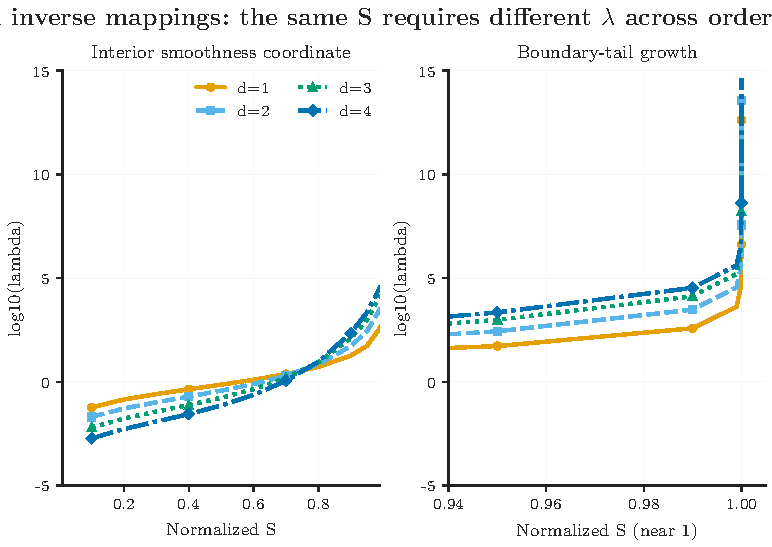
\includegraphics[width=\linewidth]{figures/sncs_smoothness_mapping.pdf}
\caption{Archived $S\mapsto\lambda$ inversions for
$n=24$, $d=1,\ldots,4$. The left panel covers the interior
of the common normalized coordinate; the right enlarges
the high-smoothness tail. A common $S$ need not imply a
common numerical penalty across difference orders.
The exact $S=1$ boundary has $\lambda=\infty$ and is
excluded from logarithmic ordinates.}
\label{fig:expanded-s-mapping}
\end{figure}

\subsection{Numerical inversion in log-penalty coordinates}
For an interior target $s$, numerical inversion solves
$F(x)=S(e^x)-s=0$ in $x=\log\lambda$. Differentiation gives
\begin{equation}
F'(x)=\frac{1}{r}\sum_j
\frac{e^x\delta_j}{(1+e^x\delta_j)^2}.
\label{eq:expanded-log-derivative}
\end{equation}
A bracket ensures that safeguarded Newton, secant,
Brent and bisection methods cannot escape the admissible
positive-penalty domain. In the tail $s\approx1$, evaluate
\[
1-S(\lambda)=\frac1r\sum_j
\frac{1}{1+\lambda\delta_j}
\]
directly rather than subtracting two nearly equal
floating-point numbers. At $s\approx0$, likewise use $S$
itself for the residual. A small residual in $F$ is not
equivalent to a small relative error in $\lambda$ at the
extreme boundaries; the benchmark records the achieved
relative error in the \emph{smaller smoothness tail}.
This inversion is one of the explicit costs of offering
a human-interpretable smoothness interface.

\subsection{Statistical selection is not a change of estimator}
For a fixed reference mean, let $C(\lambda;\mu)$ denote
one of the already established CV, GCV, AICc, BIC
or conditional Gaussian marginal-likelihood scores
\cite{cortes2017smoothness}. For example, classical
leave-one-out CV can be evaluated through
the fixed-$\mu$ smoother diagonal:
\begin{equation}
\operatorname{CV}(\lambda)
=\frac1n\sum_{i=1}^{n}
\left(\frac{y_i-\widehat\tau_i}{1-h_{ii}}\right)^2,
\qquad h_{ii}=(H_\lambda)_{ii};
\label{eq:expanded-cv}
\end{equation}
and GCV is proportional to
$n\|y-\widehat\tau\|_2^2/[n-\nu_\lambda]^2$.
AICc and BIC use the model's conditional EDF in their
information penalties; MLE profiles a Gaussian
variance-component likelihood conditional on the
specified or plug-in reference difference mean.
The criteria have different numerical scales.

Define $\widetilde C(s;\mu)=C(\Lambda_d(s);\mu)$.
As a mathematical change of variables, global minima
agree when the entire domains and boundary conventions
are treated identically:
\begin{equation}
\arg\min_{s\in[0,1]}\widetilde C(s;\mu)
=S\!\left(\arg\min_{\lambda\in[0,\infty]}
C(\lambda;\mu)\right),
\label{eq:expanded-equiv}
\end{equation}
under the appropriate set-valued interpretation.
For an interior differentiable score,
\[
\frac{\mathrm d\widetilde C}{\mathrm ds}
=\frac{C'(\lambda)}{S'(\lambda)}
=\frac{\mathrm dC/\mathrm d\log\lambda}
       {\mathrm dS/\mathrm d\log\lambda}.
\]
Stationary points are therefore not created by the
coordinate change. However, \emph{finite grids} in $s$
and in $\log\lambda$ generally sample different penalties;
a different numerical minimizer can reflect discretization,
not a change in the underlying statistical criterion.
Our experiments explicitly separate these cases.

\paragraph{Reference-mean caveat.}
When fitting, the package permits a fixed numeric $\mu$
or the observed-difference plug-in
$\widehat\mu=\operatorname{mean}(D_dy)$.
The public Gaussian MLE selector permits \texttt{mu="data"};
classical CV/GCV/AICc/BIC require a fixed numeric $\mu$.
For the data-derived comparison, the numeric estimate
is computed from \emph{training data only} and then
held fixed inside the classical criterion.
This is not the exact CV that would refit $\mu$ at every
leave-one-out deletion, nor joint MLE of $(\mu,\lambda)$.

\section{Reproducible Python implementation}
\label{sec:expanded-software}
The companion open-source \texttt{trendestimation} Python library
(version \texttt{0.1.0a0} at the evaluated snapshot) is itself
a practical outcome: it exposes Guerrero-inspired \emph{smoothness}
as a controllable coordinate while retaining the conventional
penalty $\lambda$ for compatibility. We distinguish this
software design and numerical implementation from the already
known statistical PLS method and classical selectors.
We do not claim that this is the first software package for
Whittaker--Henderson smoothing.

\subsection{Public API and reproducible usage}
A reusable \texttt{TrendSmoother(n, order=d)} object constructs
the difference operator and spectral decomposition once.
The user may prescribe a normalized target $s$, invert it to
a penalty and then fit; alternatively, a criterion selects
the penalty on either coordinate. The following minimal
example shows both workflows and the values returned:
\begin{quote}
\begin{verbatim}
from trendestimation import TrendSmoother, select_lambda

smoother = TrendSmoother(len(y), order=2)

# Prescribe normalized smoothness
lam = smoother.lambda_for_smoothness(0.86)
controlled = smoother.fit(y, lambda_=lam, mu=0.0)
print(controlled.smoothness)

# Or select an existing criterion in S coordinates
chosen = select_lambda(
    smoother, y, criterion="gcv", mu=0.0,
    search_space="smoothness",
)
trend = smoother.fit(
    y, lambda_=chosen.lambda_, mu=0.0,
).trend
print(chosen.lambda_, chosen.smoothness)
\end{verbatim}
\end{quote}
The criterion itself is unchanged; \texttt{search\_space}
chooses the numerical coordinate of its candidate search.
The returned \texttt{lambda\_} can be passed to
\texttt{fit}, while \texttt{smoothness} reports the
trace-normalized attained value. The implementation
also returns the evaluated penalty grid, scores, and
requested coordinate grid for auditing.
The current default public \texttt{TrendSmoother} uses
the reusable spectral backend; the benchmarked dense
and banded variants are not all automatic public
defaults selected by a benchmark ranking.

\subsection{Backend differences and caching}
The seven numerical implementations evaluated in the
large factorial are fresh dense solves, cached dense
solves, general banded solves, dense Cholesky,
banded Cholesky, symmetric eigendecomposition of
$Q_d$, and full SVD of $D_d$.
These are distinct linear algebra backends, \emph{not}
seven statistically different smoothers.

The full SVD expresses the penalty eigenvalues through
the squared singular values of $D_d$.
Once $y$ and a fixed $\mu$ have been projected,
evaluating traces and degrees of freedom for an additional
$\lambda$ costs only a sum over eigenvalues.
For a full reconstructed curve, the transformed spectral
coefficients must also be mapped back to $n$ coordinates.
Therefore a single EDF evaluation, one full fitted trend,
an entire CV grid including leverages, and multiple
independent searches are different timing problems.
A banded $I+\lambda Q_d$ admits sparse-band storage
and specialized factorization, often attractive for
single fits or larger $n$ \cite{weinert2007wh}.

\begin{table}[tbp]
\centering\footnotesize
\caption{Computational activities and what must be charged.
The table is methodological rather than a measured timing
ranking. $M$ is the penalty-candidate count and $R$
the number of series. Reused work must be charged
once in an end-to-end comparison.}
\label{tab:expanded-costs}
\begin{tabular}{p{.19\linewidth}p{.34\linewidth}p{.34\linewidth}}
\toprule
Task & Preprocessing and repeated work & Fair comparison criterion\\
\midrule
One fixed trend
& Build $Q_d$ or its band; solve for one $\lambda$
& Fit and setup time, agreement in $\widehat\tau$\\
One scalar criterion
& Compute fitted residuals and required EDF/leverage or likelihood diagnostics
& Score validity and total evaluation time\\
Full $M$-point search
& Prepare backend; evaluate $M$ objective scores
& Identical candidates, all scores valid\\
$R$ reused searches
& Share spectrum, candidate inversions or factorization
& Charge common preparation once\\
$S^{-1}(s)$ only
& Reuse prepared positive eigenvalues; iterate scalar root
& Tail error, failure rate and microseconds\\
\bottomrule
\end{tabular}
\end{table}

\subsection{Grid reuse and algorithmic workflow}
Figure~\ref{fig:expanded-schematic} outlines the
computational workflow. Given $(n,d)$, spectral
preprocessing depends on the \emph{operator}, not
on the particular series. A common grid
$s_1,\ldots,s_M$ can be inverted once,
cached as $\lambda_1,\ldots,\lambda_M$,
and shared among selectors and observed series.
That is different from computing a fresh inverse
for each criterion evaluation. If the entire grid
is used only once, its inversion costs must be
included in the end-to-end timing. For a
separately spaced log-$\lambda$ grid, the
candidate points differ, so the selected fit may
also differ.

\begin{figure}[tbp]
\centering
\setlength{\fboxsep}{8pt}
\fbox{\begin{minipage}{.91\linewidth}
\centering\small
{\bfseries Data and difference order $(y,n,d,\mu)$}\\[3pt]
$\Downarrow$\\[3pt]
{\bfseries Prepare $D_d$, spectral values or banded factorization}\\[3pt]
$\Downarrow$\\[3pt]
\begin{tabular}{p{.39\linewidth}|p{.39\linewidth}}
\textbf{Controlled $s$} & \textbf{Criterion selection}\\
$s\mapsto\Lambda_d(s)$ & $s$ grid or $\lambda$ grid\\
One safeguarded inverse & Optional shared inverse grid\\
\end{tabular}\\[5pt]
$\Downarrow$\\[3pt]
{\bfseries Same PLS fit at selected $\lambda$:
$(\widehat\tau,\lambda,S,\nu_\lambda)$}\\[3pt]
$\Downarrow$\\[3pt]
{\bfseries Save raw scores, selections, machine metadata,
numeric validity, and plots independently}
\end{minipage}}
\caption{Reusable software path for controlled smoothness
and criterion-based selection. Native-$S$ and once-mapped
$S\to\lambda$ grids are equivalent when their candidates
match; a separate log-penalty grid generally is not.
Each panel of the empirical application reads previously
saved selections without repeating benchmark timings.}
\label{fig:expanded-schematic}
\end{figure}

\subsection{Design for independent reproduction}
The repository separates numerical data production,
statistical analysis and figure rendering. The
80,640-trial Windows CSV and environment file, the
seed-paired solver records, and the scalar root-finding
results have been committed independently of all
PDF/SVG/PNG outputs. The plotting scripts verify
SHA-256 digests of the numeric archive and reconstruct
curves at \emph{stored} $(\lambda,\mu)$.
Thus a journal reader may change the color palette or
replace a figure layout without rerunning data-generating
simulations or hardware-sensitive timing experiments.
The independent original draft and complete experiment
matrices remain available as supplementary material.

\section{Design of the archived numerical studies}
\label{sec:expanded-design}
We now describe the computational studies in enough detail
to distinguish a statistically meaningful result from a
mere timing difference. Experiments were performed
before figure rendering and their original CSVs are
reused verbatim.

\subsection{Full-factorial backend and search comparison}
The author's Windows full-factorial experiment contains
80,640 recorded search records, not 80,640 statistically
independent series. It crosses $n\in\{24,48\}$,
orders $d=0,\ldots,5$, fixed reference means
$\mu\in\{0,0.15\}$, five scores (CV, GCV,
AICc, BIC and conditional Gaussian MLE),
seven backends, and $R\in\{1,3,8\}$ independent
series per workload with cold and shared preparation.
Two seeds, seven timing repetitions and one
BLAS thread were used. The archived environment
records Windows, Python 3.11, NumPy 2.4.6,
SciPy 1.17.1 and the OpenBLAS version.

The reference grid has seventeen $S$ targets:
the deciles between 0 and 1, plus six values
concentrated in the near-one tail from $0.95$
through $1-10^{-12}$. The exact endpoints
are analytic; CV/GCV at the $S=0$
interpolating limit need not admit a finite
ordinary value, and Gaussian marginal MLE
at $d=0$ is not applicable under the adopted model.
A computational record failing parity with the
spectral score is identified as invalid, not
allowed to win because its measured runtime
happened to be short.

There are five \emph{selection} policies of interest:
(i) full-grid native-$S$ search with an inverse
at each candidate; (ii) one-time mapped-$S$
penalty grid followed by $\lambda$-based search;
(iii) a direct finite log-$\lambda$ grid;
(iv) bounded local continuous optimization in
$S$; and (v) bounded local continuous optimization
in $\log\lambda$. The first two evaluate
\emph{identical} candidates; the third does
not, and the two continuous searches use a
variable number of objective evaluations.
Local continuous minima are \emph{not} evidence
of global optimality.

\subsection{Independent-seed solver inference}
A second author-run Windows study measures
preparation plus $M$ complete fitted curves
rather than a scalar trace or criterion.
It uses 20 independently seeded data sets
per predeclared workload and five randomized
technical timing blocks per seed.
For each paired solver comparison, let
$t_{a,i}$ and $t_{b,i}$ be the median full-task
times over timing blocks for data seed $i$.
The primary effect is a geometric mean time ratio
\[
R_{a/b}=\exp\left[
  \frac1N\sum_{i=1}^N\log
  \left(\frac{t_{a,i}}{t_{b,i}}\right)
\right].
\]
Values above one favor the denominator method.
Pointwise 95\% percentile bootstrap intervals
resample data seeds; two-sided paired sign-flip
tests are Holm-adjusted across the predeclared
comparison family. The same-host timing blocks
and the $M$ fitted penalties are \emph{not}
independent inferential units.
Sign-flip inference relies on the exchangeability/
symmetry assumption for paired log differences,
and all conclusions remain conditional on the
recorded hardware and software environment.

\subsection{Four root finders in float64}
The inversion experiment examines Brent, bracket-
safeguarded Newton, bracket-safeguarded secant and
bisection with $n=30,60,120$, $d=0,1,2,3$,
eleven targets from $10^{-14}$ to $1-10^{-14}$,
and 35 randomized timing blocks per method and
target. Every method receives the \emph{same}
already prepared smoothness spectrum.
Outcomes include successful latency, convergence
failure, iterations, function and derivative
evaluations, and tail accuracy. The $d=0$
analytic identity-spectrum inverse is recorded
but excluded from numerical-root comparisons.
These are technical timing replicates on one
host, not 35 independent data sets; accordingly
they do not receive artificial inferential
$p$ values.

\section{Computational results}\label{sec:expanded-results}
\subsection{Grid coordinate, method and reference mean}
Table~\ref{tab:expanded-coordinates} reproduces
the recorded Windows subset at $n=48$,
$d=2$, $R=1$, SVD, comparing every
selection criterion and both fixed reference
means. The reported unit is milliseconds.
The native-$S$ and premapped-$S$ searches
select exactly the same $S$ values because
the finite candidate set is identical.
In contrast, the independently sampled
log-penalty grid changes interior candidates
and occasionally changes the selected value.
Its lower runtime therefore does \emph{not}
establish a better way to find the same
finite-grid statistical estimator.

\begin{table}[tbp]
\centering\scriptsize
\caption{Recorded 17-point Windows complete-search
timings (ms), fixed $n=48,d=2,R=1$, spectral
SVD, two seeds. The first two policies share
all penalty candidates; log-$\lambda$ has
different interior candidates. The final column
shows its selected normalized smoothness and is
included to make non-equivalence visible.
Only numerically valid archive records appear.}
\label{tab:expanded-coordinates}
\resizebox{\linewidth}{!}{\begin{tabular}{llrrrrr}
\toprule
Fixed $\mu$ & Criterion & $S_{\mathrm{native}}$ & Native $S$ & Mapped $\lambda$ & Log-$\lambda$ & $S_{\log\lambda}$ \\
\midrule
0.00 & CV & 0.850 & 2.004 & 1.879 & 0.545 & 0.887 \\
0.00 & GCV & 0.850 & 1.851 & 1.800 & 0.426 & 0.887 \\
0.00 & AICc & 0.900 & 1.887 & 1.810 & 0.458 & 0.887 \\
0.00 & BIC & 0.100 & 2.016 & 1.810 & 0.449 & 0.100 \\
0.00 & MLE & 0.800 & 3.477 & 2.035 & 0.515 & 0.818 \\
0.15 & CV & 0.750 & 1.962 & 1.869 & 0.580 & 0.750 \\
0.15 & GCV & 0.750 & 1.933 & 1.765 & 0.432 & 0.750 \\
0.15 & AICc & 0.800 & 1.876 & 1.781 & 0.439 & 0.750 \\
0.15 & BIC & 0.100 & 1.909 & 1.791 & 0.464 & 0.100 \\
0.15 & MLE & 0.550 & 2.033 & 1.850 & 0.525 & 0.458 \\
\bottomrule
\end{tabular}
}
\end{table}

\begin{figure}[tbp]
\centering
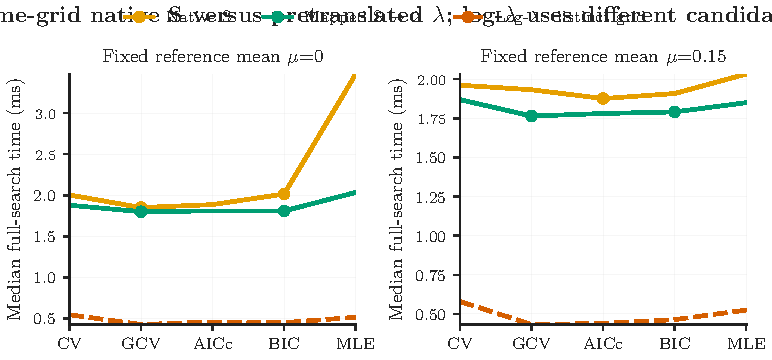
\includegraphics[width=\linewidth]{figures/sncs_coordinate_methods.pdf}
\caption{Recorded end-to-end selection time for
each criterion under $\mu=0$ and $\mu=0.15$.
Native $S$ and premapped $S\to\lambda$
operate on the same seventeen candidates.
The distinct log-$\lambda$ grid is shown
as a timing reference rather than a
matched-estimator competitor.}
\label{fig:expanded-coordinate-times}
\end{figure}

For example, in the recorded $\mu=0$
subset the CV native-$S$ search took
2.004\,ms versus 1.879\,ms for its
pretranslated counterpart; for MLE the
corresponding values were 3.477\,ms
and 2.035\,ms. These are
\emph{measured}, not modelled complexities.
Moreover, when all five criteria shared
one translated grid, the recorded sum
was 11.234\,ms for native-$S$ search
versus 3.980\,ms for
\emph{once-translated plus five backend
searches}: a descriptive ratio of 2.823.
That accounting charges the common
inverse grid only once. Its benefit
does not imply that translating a grid
is worthwhile for just one inverse target.

\begin{figure}[tbp]
\centering
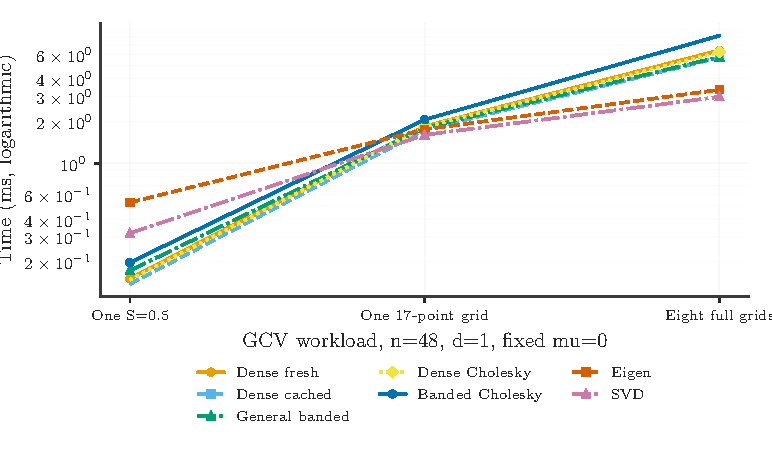
\includegraphics[width=.48\linewidth]{figures/windows_full_s_workloads.pdf}
\hfill
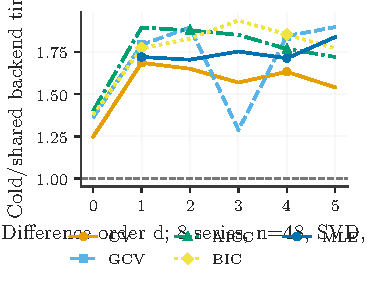
\includegraphics[width=.48\linewidth]{figures/windows_full_s_reuse_d.pdf}
\caption{Previously archived author-Windows
80,640-record study. Left: one scalar score,
one complete selection, and repeated searches
with backend-specific costs. Right: cold
versus shared preprocessing across
$d=0,\ldots,5$. The backends' validity
filters and exact sample settings are
provided in the reproducible archived
source; the two panels should not be
read as cross-hardware generalizations.}
\label{fig:expanded-workload-reuse}
\end{figure}

\begin{figure}[tbp]
\centering
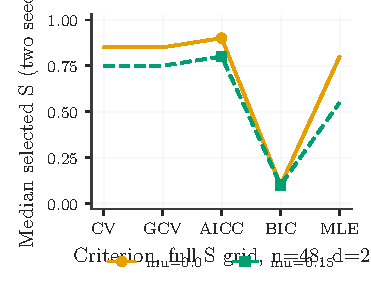
\includegraphics[width=.48\linewidth]{figures/windows_full_s_means.pdf}
\hfill
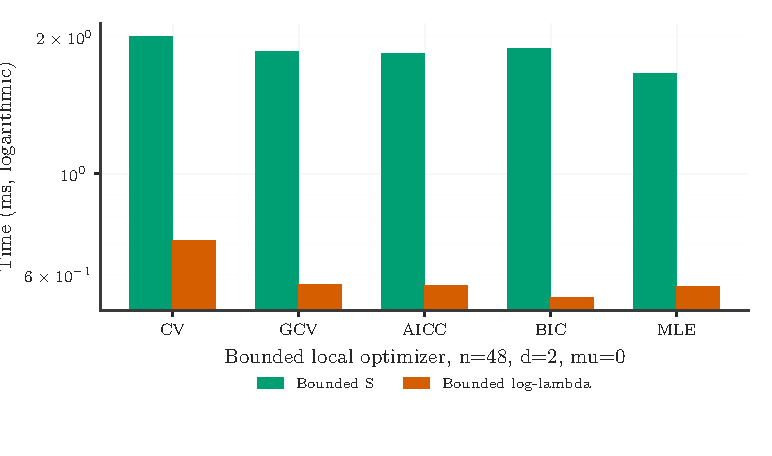
\includegraphics[width=.48\linewidth]{figures/windows_full_s_bounded.pdf}
\caption{Archived factorial comparisons:
left, selected $S$ across the five statistical
criteria under $\mu=0$ and $\mu=0.15$
for the matched candidate grid; right,
bounded \emph{local} searches over
$S$ versus $\log\lambda$.
These are separate inferential and
computational questions. A bounded
optimizer has no guaranteed global
minimum in either coordinate.}
\label{fig:expanded-mu-local}
\end{figure}

The same factorial records distinguish
seven numerical backends and all
difference orders; numerical failures
at extreme finite penalties were
screened \emph{before} a timing winner
was declared. This is particularly
important for higher order penalties:
an invalid fast dense solve does not
beat a slower accurate spectral
score. Full all-cell results, numerical
validity flags and reproducibility
metadata remain available for
inspection in the companion repository.

\subsection{Which backend is preferable for full trends?}
Table~\ref{tab:expanded-solver-orders}
reports seed-paired Windows measurements
for distinct difference orders,
a nonzero reference mean, and
several numbers of fitted curves.
These are actual full-trend timings,
not the score-only results above.
The 95\% intervals are \emph{pointwise}
bootstrap intervals; Holm-adjusted
$p$ values address the full predeclared
family of 63 solver-pair/workload
comparisons, rather than independent
tests chosen after observing the results.
Banded Cholesky is a distinct
specialized algorithm, not a new
name for the older general-banded solve.

\begin{table}[tbp]
\centering\footnotesize
\caption{Paired total-time ratio SVD/BChol
for archived full-trend computations:
ratio $>1$ favors banded Cholesky;
ratio $<1$ favors SVD. The interval is
seed-bootstrap pointwise 95\%;
Holm $p$ covers the complete
recorded family of comparisons.
$M$ is the number of fitted penalties.}
\label{tab:expanded-solver-orders}
\resizebox{\linewidth}{!}{\begin{tabular}{rrrrrll}
\toprule
$n$ & $d$ & $M$ & $\mu$ & SVD/BChol & 95\% pointwise CI & Holm $p$ \\
\midrule
96 & 1 & 16 & 0.00 & 2.205 & [2.193, 2.216] & 0.00315 \\
96 & 2 & 16 & 0.00 & 2.093 & [2.084, 2.101] & 0.00315 \\
96 & 2 & 16 & 0.15 & 2.103 & [2.097, 2.109] & 0.00315 \\
96 & 3 & 16 & 0.00 & 1.731 & [1.723, 1.742] & 0.00315 \\
96 & 5 & 16 & 0.00 & 1.168 & [1.163, 1.174] & 0.00315 \\
32 & 2 & 1 & 0.00 & 1.554 & [1.541, 1.568] & 0.00315 \\
32 & 2 & 64 & 0.00 & 0.419 & [0.417, 0.421] & 0.00315 \\
\bottomrule
\end{tabular}
}
\end{table}

\begin{figure}[tbp]
\centering
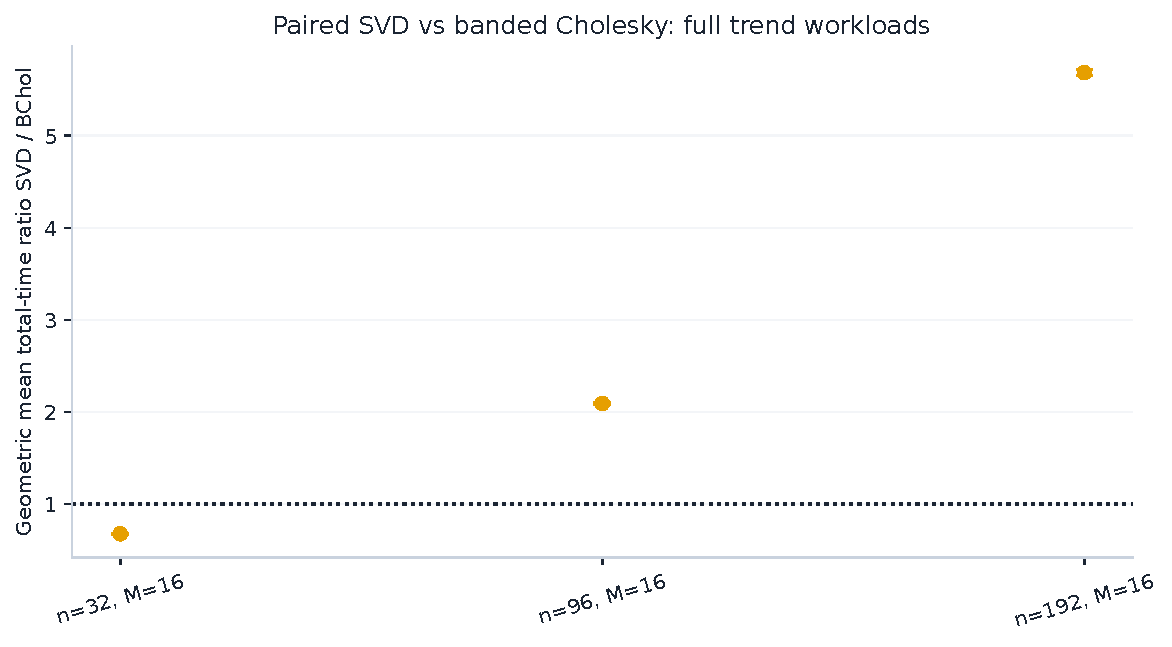
\includegraphics[width=.86\linewidth]{figures/final_solver_inference.pdf}
\caption{Archived seed-level paired time ratios
for selected full-curve workloads.
The dashed horizontal reference of one
denotes equal elapsed time, and the
intervals are pointwise, not simultaneous.
Neither a single backend nor a single
configuration is always preferred.}
\label{fig:expanded-paired-fig}
\end{figure}

The physical effect of reuse is central:
a prepared spectral transform makes
repeated $(\lambda,d)$ evaluations cheap,
while a specialized banded factorization
can avoid expensive dense preparation
for small numbers of full curves.
For example, the predeclared $d=2$
case at $n=32$ reverses its preferred
solver as the number of fitted
penalties grows from one to 64.
We do not extrapolate this crossover
to other numerical precision,
sample sizes or hardware.

\subsection{Accuracy before inversion speed}
The archived inversion results recorded
528 $(n,d,s,\text{method})$ case summaries
and no failures across their 35
technical repetitions per case.
This statement concerns precisely the
tested float64 targets and tolerances;
it does not guarantee success for every
representable $s$ or penalty spectrum.

\begin{table}[tbp]
\centering\footnotesize
\caption{Measured Brent, Newton, secant,
and bisection latency, iteration count,
failure count and maximum relative
smoothness-tail error for $n=120,d=2$
at $S=0.5$ and $S=0.99$.
All values are read from the author's
recorded float64 benchmark and require
a precomputed smoothness spectrum.
The analytic $d=0$ case is excluded.}
\label{tab:expanded-root}
\resizebox{\linewidth}{!}{\begin{tabular}{llrrrr}
\toprule
$S$ & Inversion method & Median $\mu$s & Fail / trials & Iterations & Max rel. tail error \\
\midrule
.5 & brentq & 91.50 & 0/35 & 10.0 & 1.8e-15 \\
.5 & newton & 88.30 & 0/35 & 5.0 & 2.2e-16 \\
.5 & secant & 157.70 & 0/35 & 24.0 & 1.1e-15 \\
.5 & bisect & 292.00 & 0/35 & 45.0 & 1.4e-13 \\
.99 & brentq & 93.70 & 0/35 & 11.0 & 3.3e-14 \\
.99 & newton & 118.60 & 0/35 & 8.0 & 0 \\
.99 & secant & 162.80 & 0/35 & 26.0 & 1.7e-13 \\
.99 & bisect & 282.00 & 0/35 & 45.0 & 7.7e-14 \\
\bottomrule
\end{tabular}
}
\end{table}

\begin{figure}[tbp]
\centering
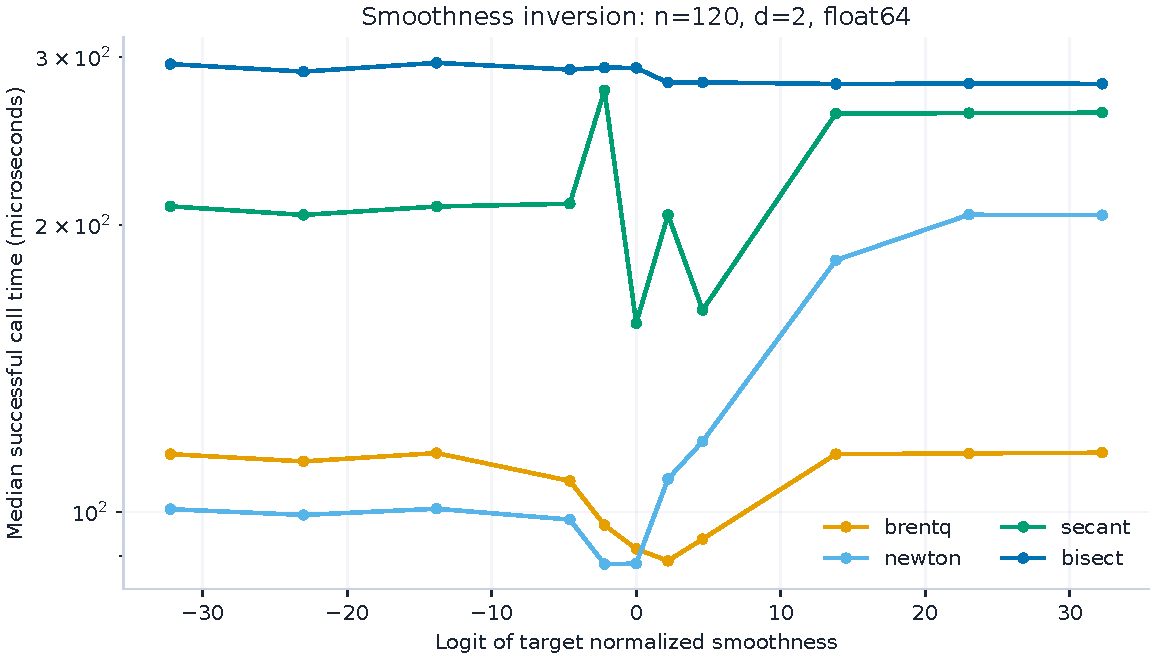
\includegraphics[width=.86\linewidth]{figures/final_inversion_speed.pdf}
\caption{Observed root inversion latencies
across $\operatorname{logit}(S)$ for
Brent, Newton, secant and bisection.
Missing or inaccurate solutions would
be explicitly recorded; only valid
outcomes contribute successful-call
medians. The plotted runtime excludes
initial spectral preprocessing.}
\label{fig:expanded-inverse-time}
\end{figure}

The distinction between full
search time and one inverse call
is important: root-finding is useful
for choosing a controlled target
but has a cost if repeated at
every candidate evaluation.
Cache a shared inverse grid
where reuse justifies it; do not
assume native-$S$ search is faster
than a numerical log-penalty search
simply because $S$ is easier to interpret.

\section{Real time-series illustrations: series, trends and selectors}
\label{sec:expanded-applications}
The final illustration is deliberately separate
from the computational timings. It tests how
the selected \emph{level} of smoothing and
the polynomial order affect an interpretable
trend rather than claiming to produce a
new stochastic forecast.

\subsection{Datasets and common candidate protocol}
We use two frozen monthly public series:
the Mauna Loa atmospheric CO$_2$ mean
($n=441$, January 1990--September 2026,
parts per million) and the monthly
US effective federal funds rate
($n=201$, January 2010--September 2026,
percent, not seasonally adjusted)
\cite{noaa2026mlo,fred2026fedfunds}.
The first contains a strong seasonal
component around long-run growth;
the second contains abrupt shifts
and extended low-rate periods.
Both are useful for illustrating how
different time scales affect
trend estimation.

For each series, the archived study
uses $d\in\{1,2,3,4\}$,
$\mu=0$ or a training-derived
$\operatorname{mean}(D_d y_{\rm train})$,
and CV, GCV, AICc, BIC,
conditional Gaussian profile MLE,
and controlled $S=0.86$.
The first five optimize their
preexisting scores over the \emph{same}
29-point finite $S$ candidate grid;
the controlled option selects $S$
by prescription rather than
minimization. Consequently a
selected $S=0.1$ or $S=0.98$
may merely be a \emph{grid
boundary} optimum.

\subsection{Observed series and four selected trends}
Figure~\ref{fig:expanded-actual-trends}
plots the \emph{observed monthly values}
and fitted trends at the
stored $d=2$, fixed $\mu=0$
parameters for four contrasting
procedures. This view makes
visible the substantive consequences
of the selection table rather
than relying on numerical RMSE
alone. Curves are recomputed
deterministically at the
saved $(\lambda,\mu)$; no
statistical criterion is
optimized to create the figure.

\begin{figure}[tbp]
\centering
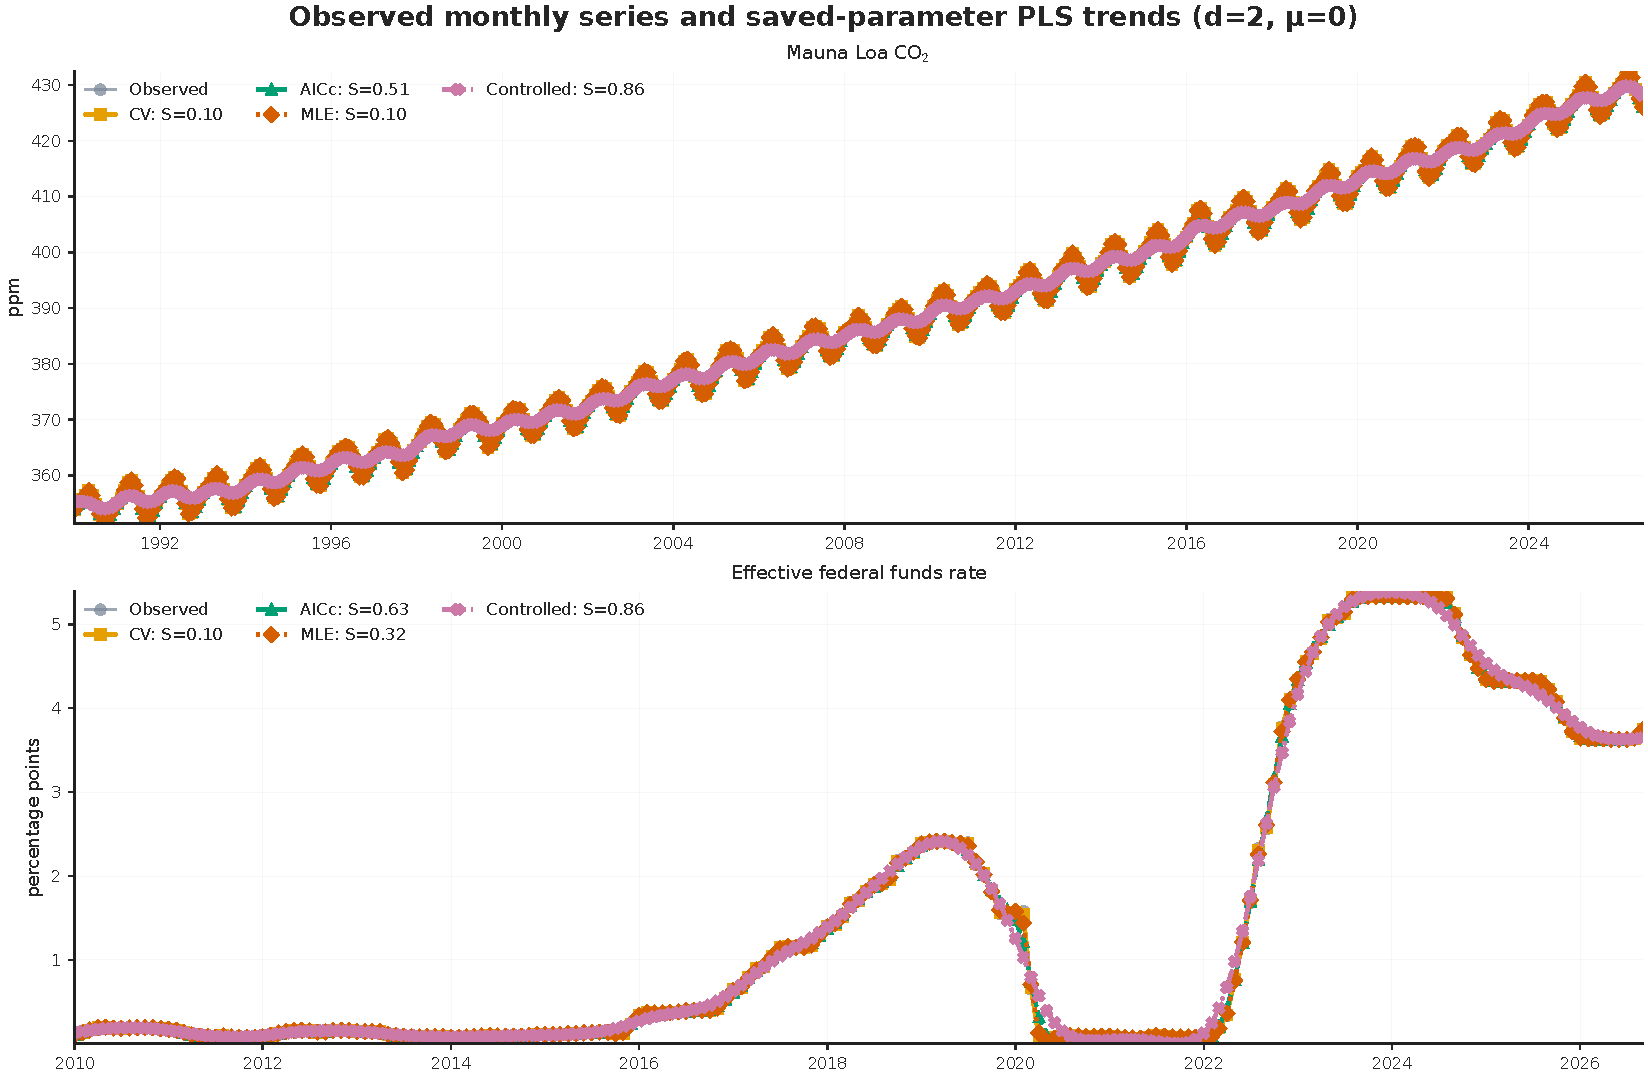
\includegraphics[width=\linewidth]{figures/sncs_observed_trends.pdf}
\caption{Frozen monthly observations
(gray) and in-sample penalized
least-squares trends for CV,
AICc, conditional MLE and
prescribed $S=0.86$,
with $d=2$ and fixed $\mu=0$.
The chosen penalty and resulting
smoothness level are drawn
from saved experiment JSON.
Coincident curves may overlap.
These are two-sided
historical smoothers, not
future forecasts.}
\label{fig:expanded-actual-trends}
\end{figure}

\begin{table}[tbp]
\centering\footnotesize
\caption{Empirical $d=2$, $\mu=0$
comparison for the two full
series. $\lambda$ and $S$
are selected in-sample;
RMSE and MAE compare a
separately extrapolated
historical 12-month holdout
against raw observations.
The 29-point search grid
is finite, and the
single-origin holdout
does not establish
predictive superiority.}
\label{tab:expanded-realdata}
\begin{tabular}{llrrrr}
\toprule
Series & Criterion & $\lambda$ & $S$ & RMSE & MAE \\
\midrule
CO$_2$ & CV & 0.0205 & 0.100 & 3.328 & 2.839 \\
CO$_2$ & GCV & 0.0205 & 0.100 & 3.328 & 2.839 \\
CO$_2$ & AICc & 0.428 & 0.509 & 3.413 & 2.930 \\
CO$_2$ & BIC & 0.0205 & 0.100 & 3.328 & 2.839 \\
CO$_2$ & MLE & 0.0205 & 0.100 & 3.328 & 2.839 \\
CO$_2$ & Controlled & 41.8 & 0.860 & 2.162 & 1.820 \\
\midrule
FEDFUNDS & CV & 0.0205 & 0.100 & 0.512 & 0.495 \\
FEDFUNDS & GCV & 0.0205 & 0.100 & 0.512 & 0.495 \\
FEDFUNDS & AICc & 1.21 & 0.634 & 0.538 & 0.522 \\
FEDFUNDS & BIC & 0.0205 & 0.100 & 0.512 & 0.495 \\
FEDFUNDS & MLE & 0.12 & 0.320 & 0.519 & 0.503 \\
FEDFUNDS & Controlled & 39.6 & 0.860 & 0.549 & 0.531 \\
\bottomrule
\end{tabular}

\end{table}

\subsection{Why the difference order matters even at equal $S$}
A simple but important geometric
point is that the same normalized
trace smoothness does not imply
the same fitted curve. At $d=1$,
the limiting zero-reference
trend is constant. At $d=2$,
it is linear; larger orders
allow correspondingly
higher-degree polynomial
null spaces. As a result,
the finite-$\lambda$ curves
with the same normalized
$S=0.86$ differ as well.
Figure~\ref{fig:expanded-orders}
plots all four orders for both
series, using the same prescribed
smoothness instead of pretending
that equal $\lambda$ values
have a comparable meaning.

\begin{figure}[tbp]
\centering
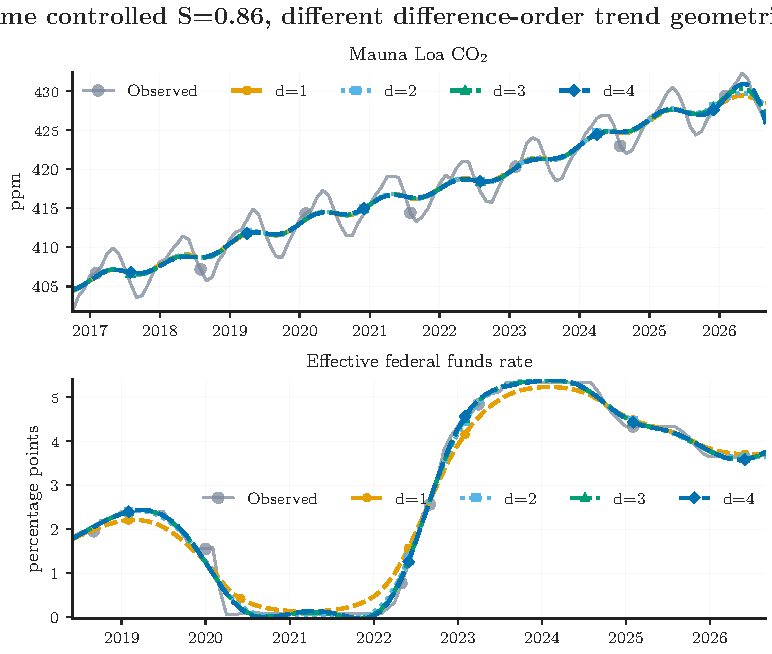
\includegraphics[width=\linewidth]{figures/sncs_orders_trends.pdf}
\caption{The most recent monthly
observations and four estimated
trends at the \emph{same}
controlled normalized
$S=0.86$ under
$d=1,2,3,4$, fixed $\mu=0$.
The variation across panels
is due to the finite-difference
order and its different
null-space geometry, not to
a change in the prescribed
fraction of trace smoothness.}
\label{fig:expanded-orders}
\end{figure}

\subsection{Criteria and data-derived reference differences}
Figure~\ref{fig:expanded-dashboard} uses
the archived selection and holdout
matrices to show two different
questions on a common $4\times6$
layout: how much smoothness is
selected, and how much
one-origin error is incurred
by the \emph{separate}
extrapolation rule.
The corresponding data-derived
$\mu$ figure, full 24-panel
trend/forecast collections,
and the most recent 120-month
CO$_2$ subset are provided
as supplementary figures.
For $\mu$ estimated from
observed differences, the
numeric value is computed
\emph{before} choosing the
penalty and separately for
each historical training window.

\begin{figure}[tbp]
\centering
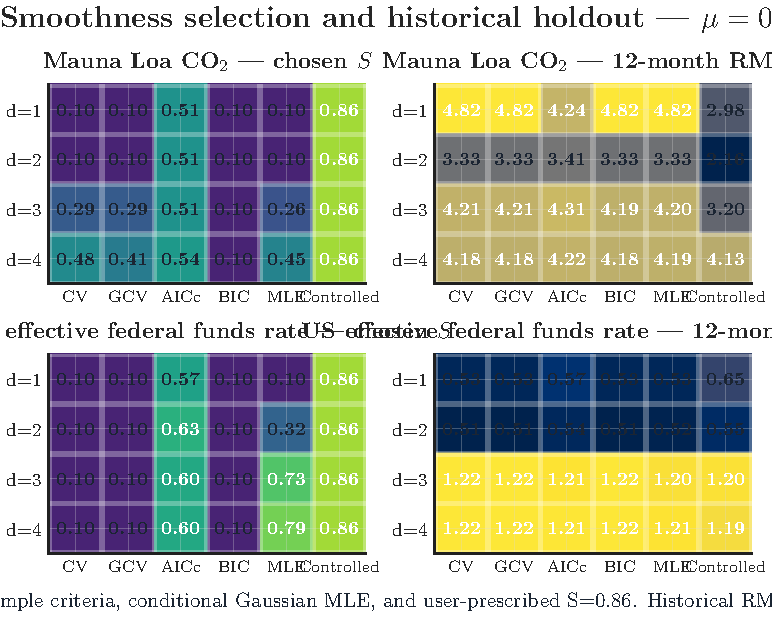
\includegraphics[width=\linewidth]{figures/sncs_compact_dashboard.pdf}
\caption{Saved smoothness
selection and historical
12-month holdout errors for
the two observed series,
four difference orders,
and six policies under
$\mu=0$. The six columns
include one prescribed
smoothness level and five
distinct in-sample
criterion objectives.
Only one historical
forecasting origin is
represented.}
\label{fig:expanded-dashboard}
\end{figure}

The extrapolation in the archive
is an explicit anchored local
polynomial fitted to the end
of each historical PLS trend,
not the PLS estimator itself.
For the historical holdout,
all mean and penalty
selections use the
training period only,
and the prediction error
is measured against
\emph{noisy observed values},
not the inaccessible
latent trend. For CO$_2$
the extrapolation has no
seasonal model; for the
federal funds rate it
does not model regime or
policy changes. Consequently
its one-origin errors
are illustrative diagnostics
and not the basis for
claiming that a particular
smoother or root algorithm
is a superior forecasting
method.


\section{Discussion, limitations and conclusion}\label{sec:sncs-conclusion}
The distinction among a smoother, its statistical tuning
criterion, and the algorithm used to evaluate that criterion
is essential. Our normalized $S$ is a trace-based order-adjusted
version of Guerrero's index; selecting $S$ directly is a useful
software abstraction, but does not create a new estimator.
For finite grids, candidate penalties must be identical before
timing methods can be interpreted as solving the same
statistical selection problem. A separately spaced
log-$\lambda$ grid is a legitimate alternative design,
but its chosen fit and selection score may differ.

The archived full-factorial Windows records quantify this
distinction across seven backends, five criteria, two fixed
means, multiple order choices and computational reuse patterns.
The independent seed-paired full-trend analysis supplies
pointwise bootstrap intervals and multiplicity-adjusted
hypothesis tests on those particular workloads. The inversion
benchmark confirms numerical accuracy for the tested targets
and reveals costs of offering the more interpretable
smoothness-first coordinate. It does not establish
hardware-independent superiority, nor should repeated
technical timings be treated as independent data seeds.
The package's default spectral solver is not claimed
to be universally faster than a specialized banded solver.

The real-data case studies illustrate two further limits.
The same $S$ need not produce the same geometric curve
under different $d$, and fitting $\mu$ from observations
changes the interpretation of conditional degrees of
freedom. Furthermore, a historical two-sided PLS trend
does not define a forecasting process; the archived
continuations depend on a separate polynomial extrapolation.
Single-origin holdout RMSE does not justify a claim of
superior future predictive accuracy. We therefore separate
the computational conclusions of this article from
forecasting-method development.

Our main practical result is a reproducible Python
implementation of smoothness-indexed PLS that links
theory, criterion selection, numerical solvers, and
archived evidence. Full high-order matrices, individual
candidate scores, complete 4$\times$6 forecasting grids,
and machine metadata are provided in the repository
rather than crowding the journal text. Future work should
investigate larger $n$, multiple hardware environments,
regularized likelihood treatments of unknown $\mu$,
and genuinely multi-origin forecasting tests.

\section*{Declarations}
\noindent\textbf{Funding and competing interests.}
To be completed and verified by the coauthors before submission.

\noindent\textbf{Data availability.}
Frozen NOAA and FRED observations, selection-result JSONs,
timing CSVs, uncertainty analyses, and rendering manifests
are archived in the companion repository.
\noindent\textbf{Code availability.}
\url{https://github.com/heri-espino/trendestimation}.
A permanently archived tagged release should be cited on submission.
\noindent\textbf{Author contributions.}
To be agreed by the coauthors.
\bibliography{bibliografia}
\end{document}
